\documentclass{article}
\usepackage[utf8]{inputenc}
\usepackage{graphicx}
\usepackage{mathtools} 
\usepackage{textcomp}
\usepackage{titling}
\usepackage{subfig}
\usepackage{amsmath}
\usepackage[parfill]{parskip}
\usepackage{xcolor}
\definecolor{LightGray}{gray}{0.9}
\usepackage{titlesec}
\setcounter{secnumdepth}{4}
\usepackage[a4paper,left=1cm,right=1cm,top=1cm,bottom=1.5cm,]{geometry}
\usepackage{eqparbox}

\title{\vspace{-2cm} EE4218 L4 - Abstract Models, Behavioral Synthesis}
\date{\vspace{-5ex}}

\begin{document}
\maketitle

\section{Abstract Models}
\subsection{Structure}
At it's highest level, a \textit{structure} is an interconnection of various components.

Formally, we define an \textit{incidence structure} as an abstract system consisting of two types of objects, and a single relationship between these types of objects. There are man

There are different kinds of incidence structures corresponding to different ways to model something.

\subsubsection{Modules/Pins + Nets + Incidence relation}
A natural way to model hardware is via \textit{modules} and \textit{nets}, with their interconnections described by \textit{incidence relations}.

\begin{figure}[htp]
    \centering
    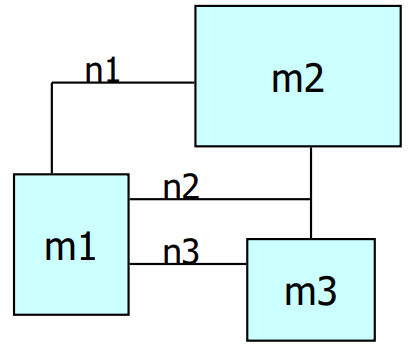
\includegraphics[width=5cm, scale=1]{S1/modulesNetsRelations.PNG}
    \caption{Modules, nets and pins}
\end{figure}

Seen in Fig1 above, we term net \textit{$n_{1}$} as being incident on modules \textit{$m_{1}$} and \textit{$m_{2}$}

\subsubsection{Hypergraph, Bipartite Graph}
Another way to model is to use graphs, where \textit{vertices} correspond to modules and \textit{edges} correspond to nets.

When a particular net $n_{i}$ is incident on a module $m_{j}$, there is an associated edge $e_{k}$ connecting $n_{i}$ and $m_{j}$,
where each of these edges denotes an incidence relation.

\begin{figure}[htp]%
    \centering
    \subfloat[\centering Hypergraph]{{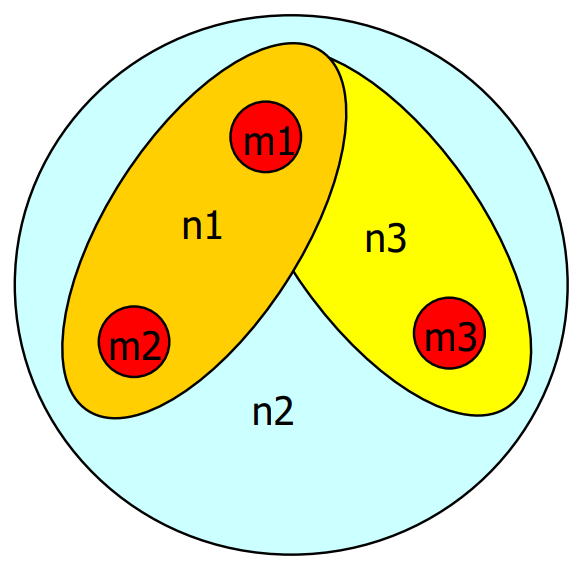
\includegraphics[width=5cm]{S1/hypergraph.PNG}}}% 
    \qquad
    \subfloat[\centering Bipartite graph]{{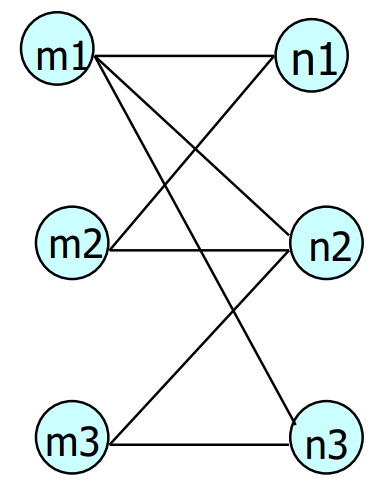
\includegraphics[width=5cm]{S1/bipartiteGraph.PNG}}}% 
    \caption{Graph-based modelling}%
\end{figure}

\begin{itemize}
    \item Hypergraph is a generalization of a graph, where any edge can join \textbf{any} number of vertices
    \item Bipartite graph is a graph where every edge connects a vertex in $U$ to one in $V$
        \begin{itemize}
            \item Notice that modules $\left\{ m_{1}, m_{2}, m_{3} \right\}$ are placed on one side,
                  nets $\left\{ n_{1}, n_{2}, n_{3} \right\}$ placed on the other side.
                  Therefore modules \textbf{cannot} be directly connected to other modules; they required a net interconnection.
                  Similarly nets \textbf{cannot} be directly connected to other nets; if they were, it would just be considered the same net!
        \end{itemize}
\end{itemize}

\subsubsection{Incidence Matrix, Netlists}
From the discussion above, we notice the idea of incidence relations. 
A natural way of representing incidence relations is to use \textit{incidence matrices}, as seen in Fig3 below.

\begin{figure}[htp]
    \centering
    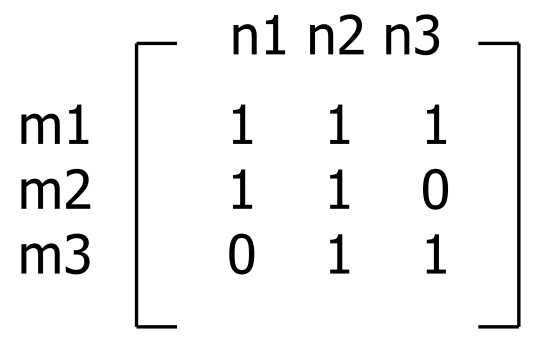
\includegraphics[width=3cm, scale=1]{S1/incidenceMatrix.PNG}
    \caption{Incidence Matrix}
\end{figure}

In practical applications, incidence matrices tend to be \textit{sparse}.
Therefore a more efficient representation is to downgrade from \textit{matrix} to a net\textit{list}. Accoridngly we have two types of netlists, \dots
\begin{itemize}
    \item Net-oriented; Enumerating all modules of a given net
    \item Module-oriented; Enumerating all nets of a given module
        \begin{itemize}
            \item \eqmakebox[things][l]{eg.}
                    $ \begin{aligned}[t]
                    &m1:n1,n2,n3\\
                    &m2:n1,n2\\
                    &m3:n2,n3
                    \end{aligned} $ 
        \end{itemize}
\end{itemize}

\subsubsection{Hierarchy}
There is the concept of \textit{hierarchy} within a structure, where submodules may be connected together to create a larger module.
\begin{itemize}
    \item \textit{Leaf} modules are \textit{primitives} (ie. Module that does not have any submodules 'within it')
        \begin{itemize}
            \item Usually primitives are used to describe something that is already available in the cell library
        \end{itemize}
    \item \textit{Non-leaf} modules are composed from a set of modules (termed it's \textit{submodules})
\end{itemize}

\begin{figure}[htp]
    \centering
    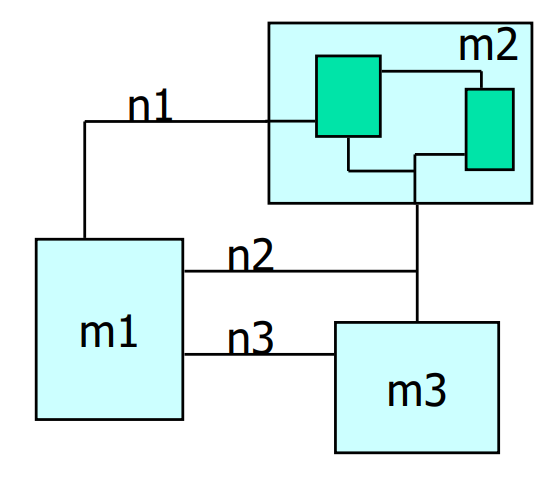
\includegraphics[width=4cm, scale=1]{S1/hierarchy.PNG}
    \caption{$m_{1}$ and $m_{3}$ are leaf modules\\
             $m_{2}$ is non-leaf module (composed of it's submodules)}
\end{figure}

\subsection{Logic Network}
\textit{Logic networks} are defined to be \textit{blocks} interconnected with \textbf{directional} nets
\begin{itemize}
    \item Each \textit{block} is modelled by a boolean function (ie. combinational logic)
    \item Since each block is implementing combinational logic, a logic network is purely \textbf{combinational}
    \item More specifically, each block is a \textit{multi-input, single-output} \textbf{leaf} module
    \item In the special case where the blocks correspond to cell library elements, we term it a \textit{mapped network}
\end{itemize}

\begin{figure}[htp]%
    \centering
    \subfloat[\centering Logic Network]{{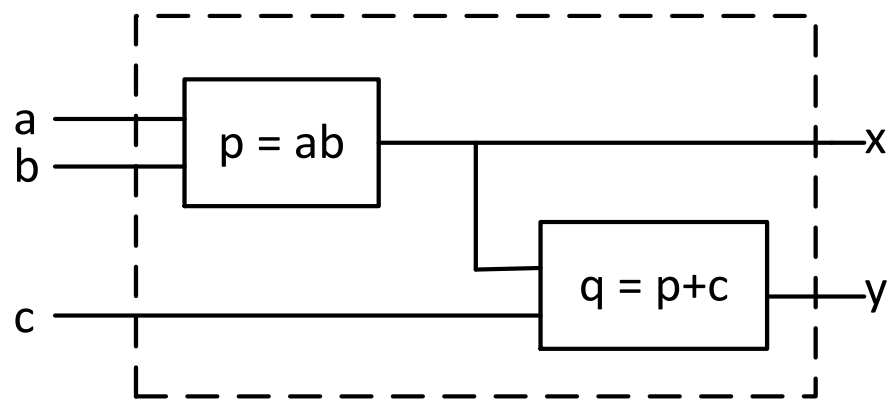
\includegraphics[width=6cm]{S1/logicNetwork.PNG}}}% 
    \qquad
    \subfloat[\centering Logic Network graph]{{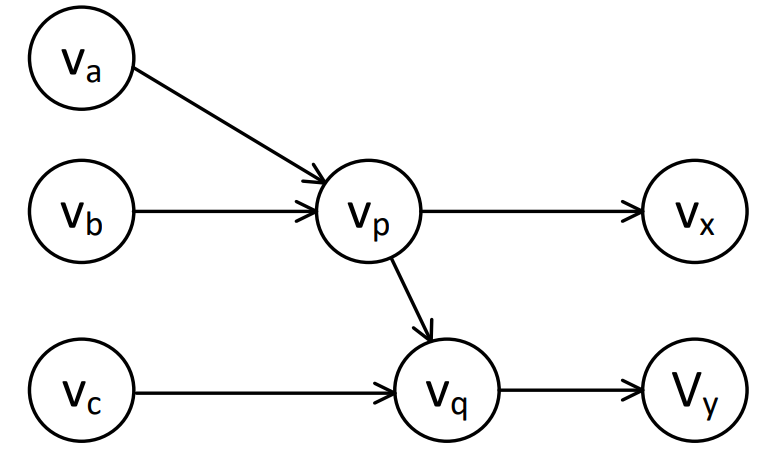
\includegraphics[width=5cm]{S1/logicNetworkGraph.PNG}}}% 
    \caption{Different ways of representing Logic Networks}%
\end{figure}

\newpage
Logic networks have structural and behavioral semantics
\begin{itemize}
    \item Structural semantics can be induced by the interconnection of blocks
    \item Behavioral semantics can be extracted from the boolean expression of each block
\end{itemize}

\subsubsection{Synchronous Logic Network}
Extends the concept of logic networks, to include synchronous elements.

To do that, we allow the edges to have weights (denoting delays).

\begin{figure}[htp]
    \centering
    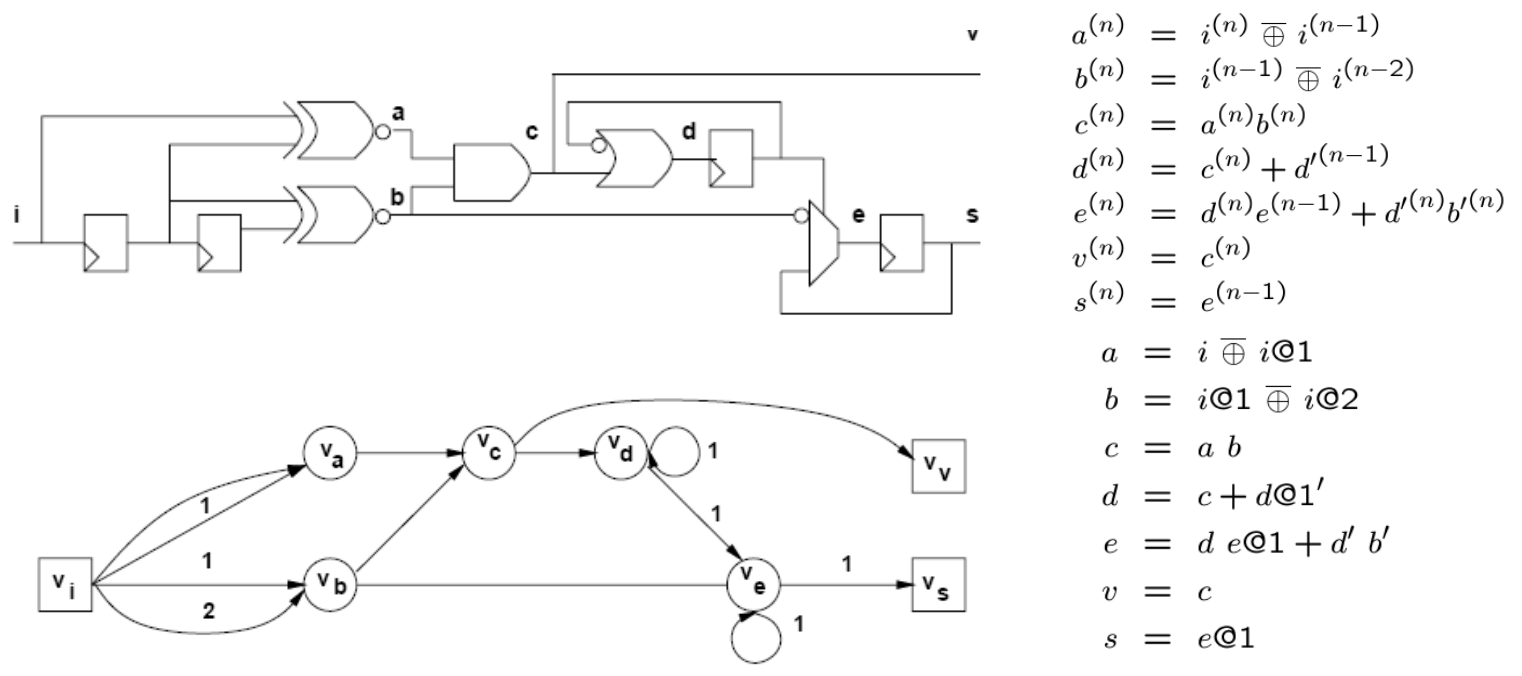
\includegraphics[width=15cm, scale=1]{S1/syncNetwork.PNG}
    \caption{Synchronous Logic Network (as seen in L3)}
\end{figure}

\subsection{Finite-State Machine}
A \textbf{purely behavioral} model.

Can be described by \dots
\begin{itemize}
    \item A set of primary input patterns \textit{X}
    \item A set of primary output patterns \textit{Y}
    \item A set of states \textit{S}
    \item Two functions \dots
        \begin{enumerate}
            \item State transition function; $\delta:X\times S \xrightarrow{} Y$
            \item Output function (Mealy); $\lambda:X\times S \xrightarrow{} Y$
            \item Output function (Moore); $\lambda:S \xrightarrow{} Y$
        \end{enumerate}
\end{itemize}

\begin{figure}[htp]%
    \centering
    \subfloat[\centering State table]{{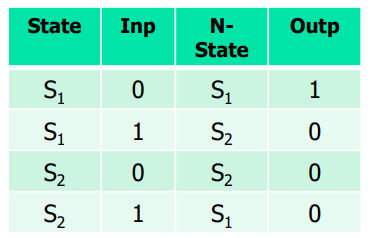
\includegraphics[width=6cm]{S1/FSM_table.PNG}}}% 
    \qquad
    \subfloat[\centering State diagram]{{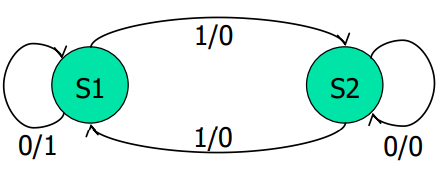
\includegraphics[width=6cm]{S1/FSM_diagram.PNG}}}% 
    \caption{Different ways of representing FSMs}%
\end{figure}

\newpage
\subsection{Dataflow Graph (DFG)}
A \textbf{purely behavioral} model, used to represent \textit{data-paths}.

Vertices represent operations, edges represent dependencies

\begin{figure}[htp]
    \centering
    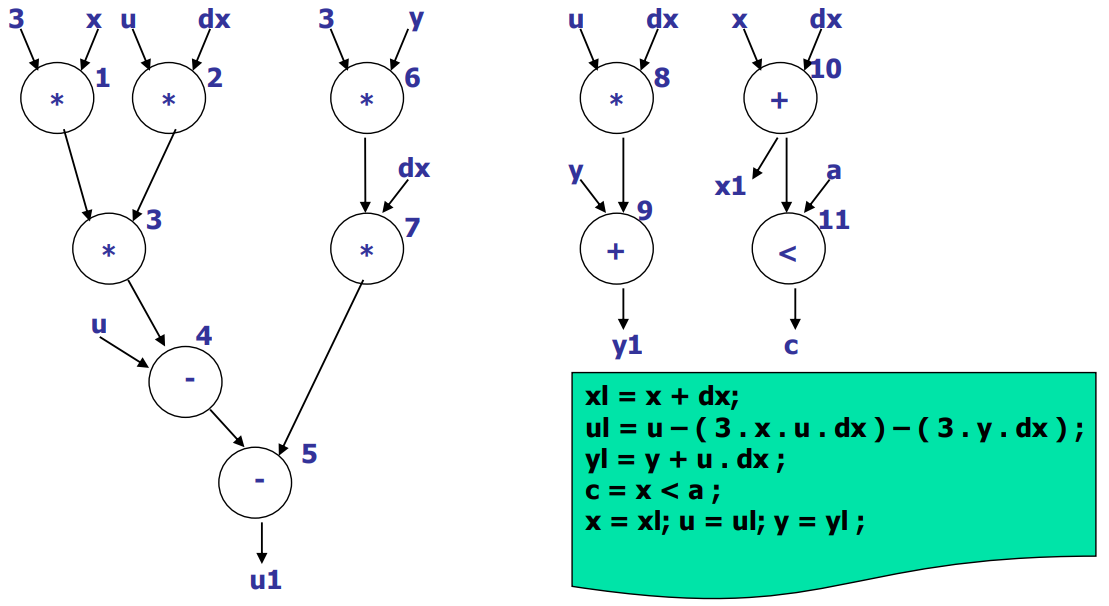
\includegraphics[width=15cm, scale=1]{S1/dataFlowGraph.PNG}
    \caption{DFG}
\end{figure}

DFG is also useful to see where registers might need to be inserted (since the results of operating on data need to be saved into memory eventually)

However, note that DFGs only say what the operations are and what the dependencies are.
It does not give us \textit{control information} (eg. some operations might only be done on a conditional basis).

\subsection{Sequencing Graph (CDFG)}
A \textbf{purely behavioral} model, used to represent \textit{data-paths} \textbf{and} \textit{control-paths} (ie. enchanced version of DFG).

Note that oftentimes the CDFG is shown without data annotations, especially when doing \textit{scheduling} (when to perform operation) or \textit{binding} (where to perform operation).

\begin{figure}[htp]
    \centering
    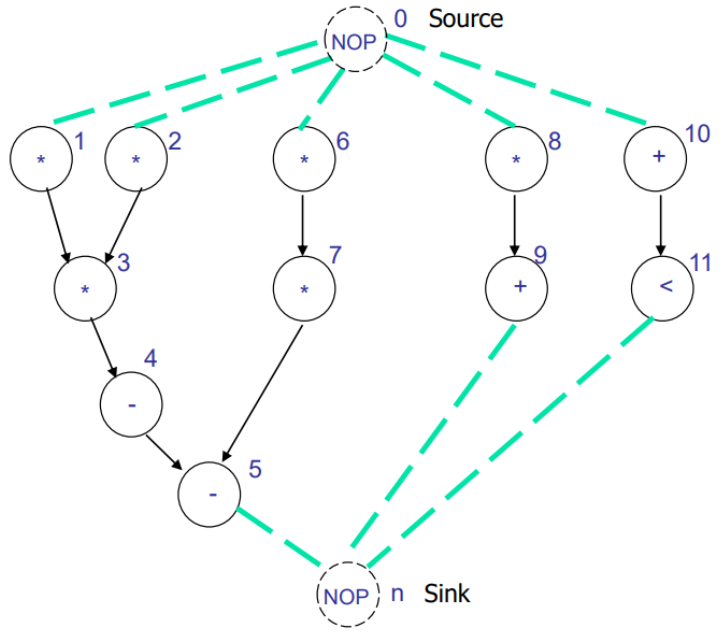
\includegraphics[width=8cm, scale=1]{S1/sequencingGraph.PNG}
    \caption{CDFG. The \textit{NOPs} mean that the hardware isn't doing anything before/after the operations}
\end{figure}

CDFG's can furthur show us \dots
\begin{itemize}
    \item Hierarchy
    \item Control-flow commands (e.g \textit{branching}, \textit{iteration})
\end{itemize}


\newpage
\subsubsection{Sequencing Graphs: Hierarchy}
What is "inside" a vertex? 

In a CDFG, vertices may contain other 'sub-vertices' (ie. operations) within them. Therefore, it performs simiar to a function call in programming.

\begin{figure}[htp]
    \centering
    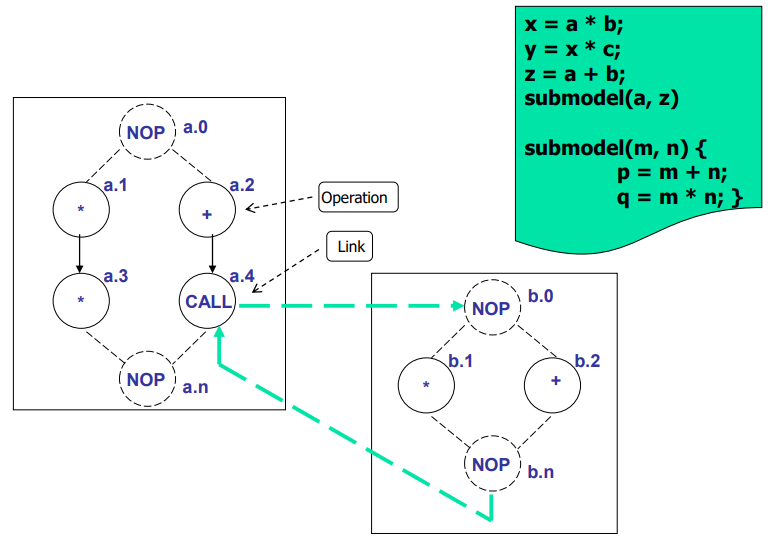
\includegraphics[width=12cm, scale=1]{S1/sequencing_hierarchy.PNG}
    \caption{"Function calls" in a CDFG}
\end{figure}

\subsubsection{Sequencing Graphs: Control Information}

\begin{figure}[htp]%
    \centering
    \subfloat[\centering Branching]{{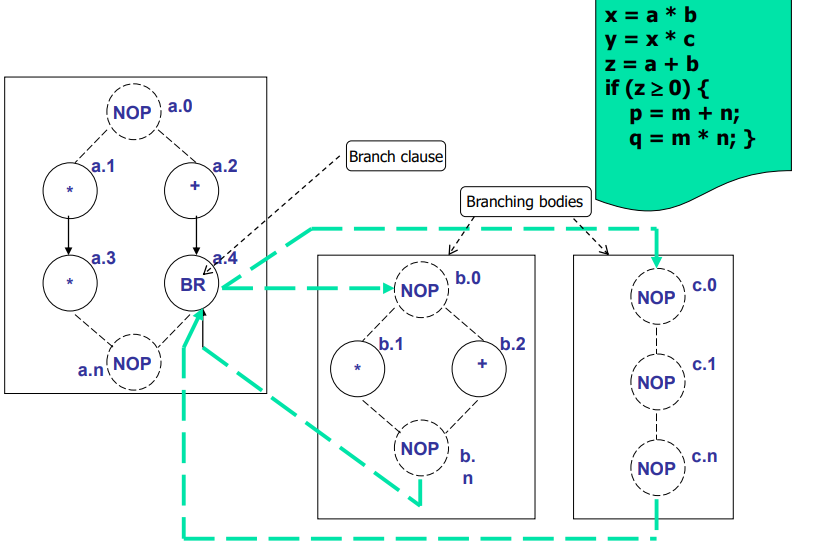
\includegraphics[width=9cm]{S1/sequencing_branching.PNG}}}% 
    \qquad
    \subfloat[\centering Iteration]{{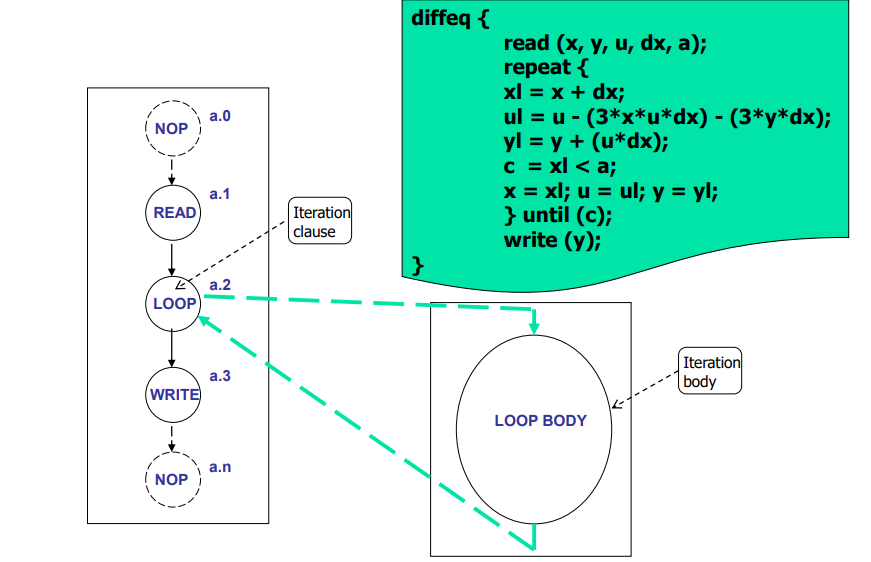
\includegraphics[width=9cm]{S1/sequencing_iteration.PNG}}}% 
    \caption{Control information in a CDFG}%
\end{figure}

\subsubsection{Sequencing Graphs: Semantics}
What can a CDFG tell us?

Vertices (representing operations) can be in either of the three states \dots
\begin{enumerate}
    \item \textit{Waiting} for execution
    \item \textit{Executing}
    \item \textit{Completed} execution
\end{enumerate}

From the CDFG's POV, a vertex can be executed as soon as all of it's \textbf{immediate} predecessors have completed execution (we term this \textit{precedence constraints}).
However, is this really true?

\begin{itemize}
    \item CDFG's are only concerned with the behavioral aspects, there is no notion of structural aspects (availability of hardware to actually execute the operation)
\end{itemize}

\newpage
\subsubsection{Vertex attributes}
What can the vertices of a CDFG tell us?
\begin{itemize}
    \item Area cost
        \begin{itemize}
            \item eg. A multiplication vertex '*' has an associated hardware area cost.
                   
                  Note that the hardware cost may not be fixed (eg. Multiplication units may be implemented combinationally or sequentially, which have different area costs)
        \end{itemize}
    \item Delay cost, furthur categorized as \dots
        \begin{itemize}
            \item Propagation delay (denoted in seconds); Corresponding to \textit{combinational} delays
             \begin{itemize}
                \item Combinational logic has no concept of 'cycles', everything is done within one 'cycle'. 
                      Therefore the concept of 'execution cycles' is not applicable to combinational logic.
             \end{itemize}
            \item Execution delay (denoted in \textit{number of cycles}); Corresponding to textit{sequential} delays
             \begin{itemize}
                \item Execution delays may be \textit{data-dependent} (eg. runtime of booth's multiplication algorithm is data-dependent)
                \item Execution delays may be \textit{bounded} (eg. branching) or \textit{unbounded} (eg. while-loops where exit condition of the loop is itself modified by the loop)
             \end{itemize}
        \end{itemize}
\end{itemize}

\subsubsection{CDFG estimates}
What area and delay estimates can we make from a CDFG?

Let's use the CDFG from Fig9 as an example (copied here for convenience)
\begin{figure}[htp]
    \centering
    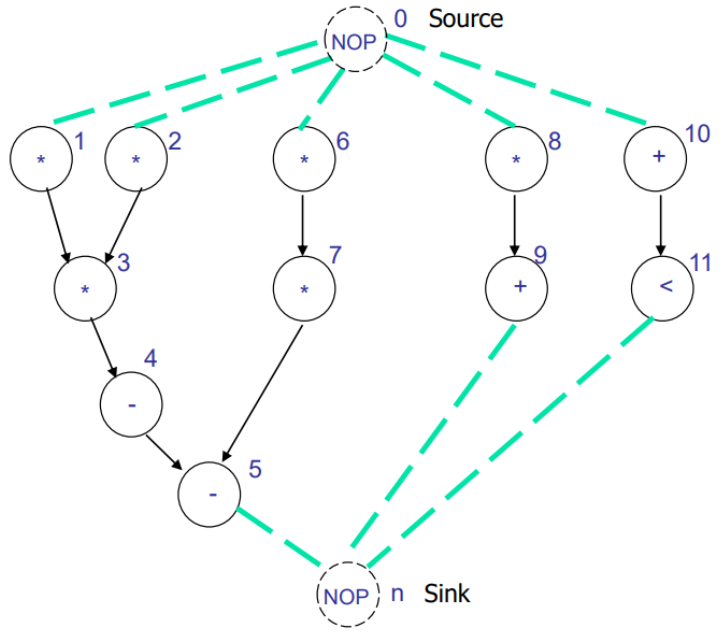
\includegraphics[width=8cm, scale=1]{S1/sequencingGraph.PNG}
    \caption{CDFG graph. Assume that area and delay are determined entirely by the ALUs and MULs}
\end{figure}

\begin{itemize}
    \item Area estimates; Only the \textbf{upper bound} is meaningful, lower bound is simply (1 ALU, 1 MUL)
        \begin{itemize}
            \item Upper bound is st. each operation has dedicated hardware (ie. no sharing of hardware resources, termed \textit{dedicated binding}).
                  Therefore, upper bound (ie. maximal area) is 6 MULs, 5 ALUs
        \end{itemize}
    \item Delay estimates
        \begin{itemize}
            \item Lower bounded by the longest path from \textit{source} to \textit{sink} \textbf{in terms of delay}.

                \begin{itemize}
                    \item Note that this is not to be confused with critical path delay of a combinational circuit (vertices of a CDFG are usually not connected back-to-back in a combinational fashion)
                    \item Furthur note that the delay is lower bounded when the area is upper bounded.
                \end{itemize}
            \item Upper bounded (meaningfully) by the scenario where only 1 ALU is available, 1 MLU is available (a meaningless delay estimate is $\infty$, where no hardware units arae available).
                \begin{itemize}
                    \item If we are upper bounded by only having 1 functional unit of each type, can we look at the CDFG and derive the optimal delay?
                          This problem is actually the \textit{scheduling problem}, and is NP-hard.
                \end{itemize}
        \end{itemize}
\end{itemize}

\newpage
\section{Behavioral Synthesis (High-Level Synthesis)}
Synthesizing \textit{behavioral} (not necessarily HDL) code rather than RTL code.

'Synthesis' in this context is not the same as Vivado's 'synthesis'.


\subsection{Behavioral Synthesis Steps}
Note that it shares many similarities with software compilation

\begin{figure}[htp]%
    \centering
    \subfloat[\centering Software compilation vs Hardware synthesis]{{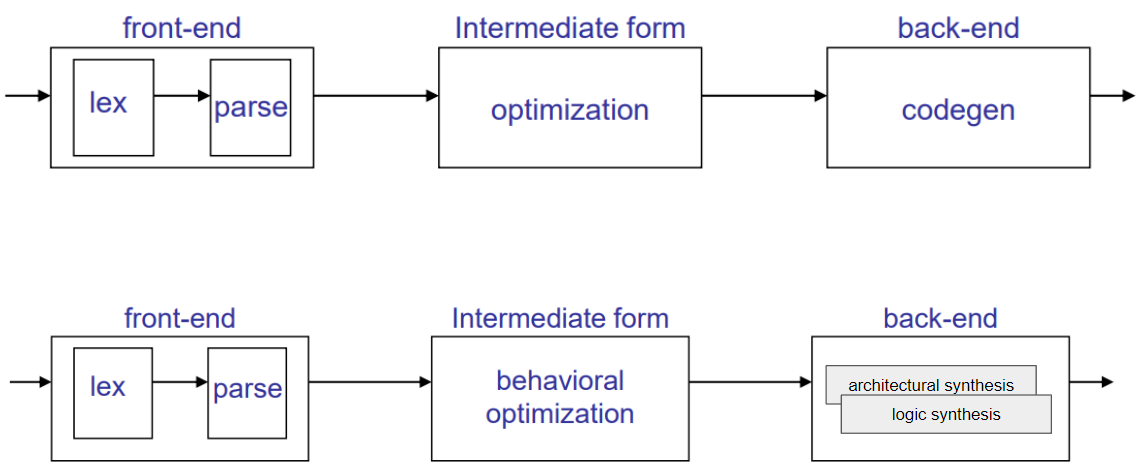
\includegraphics[width=9cm]{S2/softhardCompilation.PNG}}}% 
    \qquad
    \subfloat[\centering Simplified FPGA/ASIC design flow]{{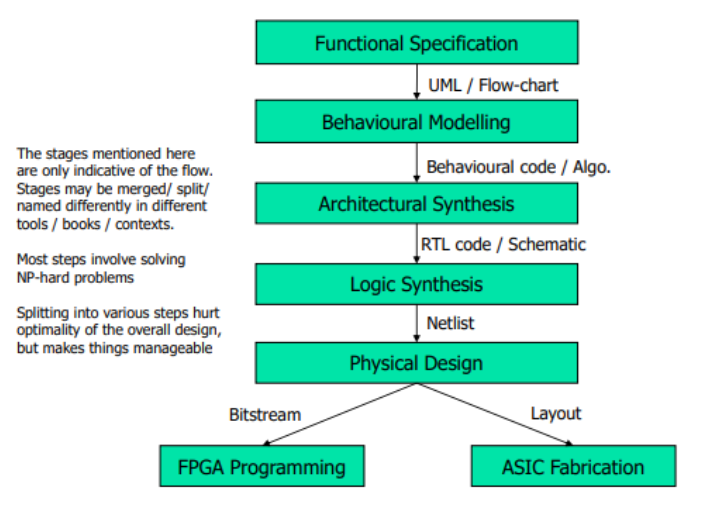
\includegraphics[width=9cm]{S2/designFlow.PNG}}}% 
    \caption{}%
\end{figure}

Software compilation \dots
\begin{enumerate}
    \item Compile program into machine form
    \item Optimize intermediate form
    \item Generate target code for architecture
\end{enumerate}

Hardware compilation \dots
\begin{enumerate}
    \item Elaborate HDL model into sequencing graph
    \item \textit{Behavioral-level optimization}; Optimize sequencing graph
        \begin{itemize}
            \item Optimize abstract models \textbf{independently} from \textit{implementation} parameters
        \end{itemize}
    \item \textit{Architectural synthesis} and \textit{optimization}; \textbf{Macroscopic} level
        \begin{itemize}
            \item Converts a \textit{behavioral} model to a macroscopic \textit{structural} model
            \item Utilizes macroscopic building blocks (Adders, Registers, \dots)
            \item Involves \textit{scheduling} (delay considerations) and \textit{binding} (area considerations)
            \item Transcompiles optimized TLM to RTL (described using HDL) design
        \end{itemize}
    \item \textit{Logic synthesis}; \textbf{Microscopic level}
        \begin{itemize}
            \item Turns RTL design into design implementation (in terms of the technology library's building blocks)
                \begin{itemize}
                    \item For ASICs, building blocks are usually gates
                    \item For FPGAs, building blocks are CLBs (which can offer higher level of functionality compared to ASICs)
                \end{itemize}
            \item Apply furthur constraints (eg. Logical port to physical pin mapping)
        \end{itemize}
\end{enumerate}

\subsection{Front-end (Lexers and Parsers)}

\subsubsection{Lexers (Lexical analysis)}
Conversion of text into meaningful \textit{lexical} tokens

\subsubsection{Parser (Syntactic analysis)}
Generates a \textit{parse tree} from lexical tokens
\begin{figure}[htp]
    \centering
    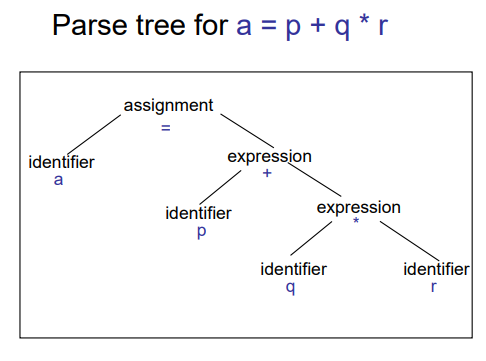
\includegraphics[width=8cm, scale=1]{S2/parseTree.PNG}
    \caption{Parse tree}
\end{figure}

\subsubsection{Semantic Analysis}
Checks if your parse tree makes \textit{semantic} sense

\begin{itemize}
    \item Data-flow and control-flow analysis
    \item Type checking
    \item Resolving and checking arithmetic and relational operators
    \item \dots
\end{itemize}

\subsection{Behavioral-level optimizations}
\textbf{Semantic-preserving} transformations aimed at simplifying the model,
Applied to parse-trees during or after their generation.

Divided into \textit{data-flow} based transformations and \textit{control-flow} based transformations \dots

\subsubsection{Some data-flow based transformations}
\begin{itemize}
    \item Tree-height reduction
        \begin{itemize}
            \item Applied to arithmetic operations only
            \item Goal is to balance the parse tree, in order to exploit hardware parallelism
            \begin{figure}[htp]
                \centering
                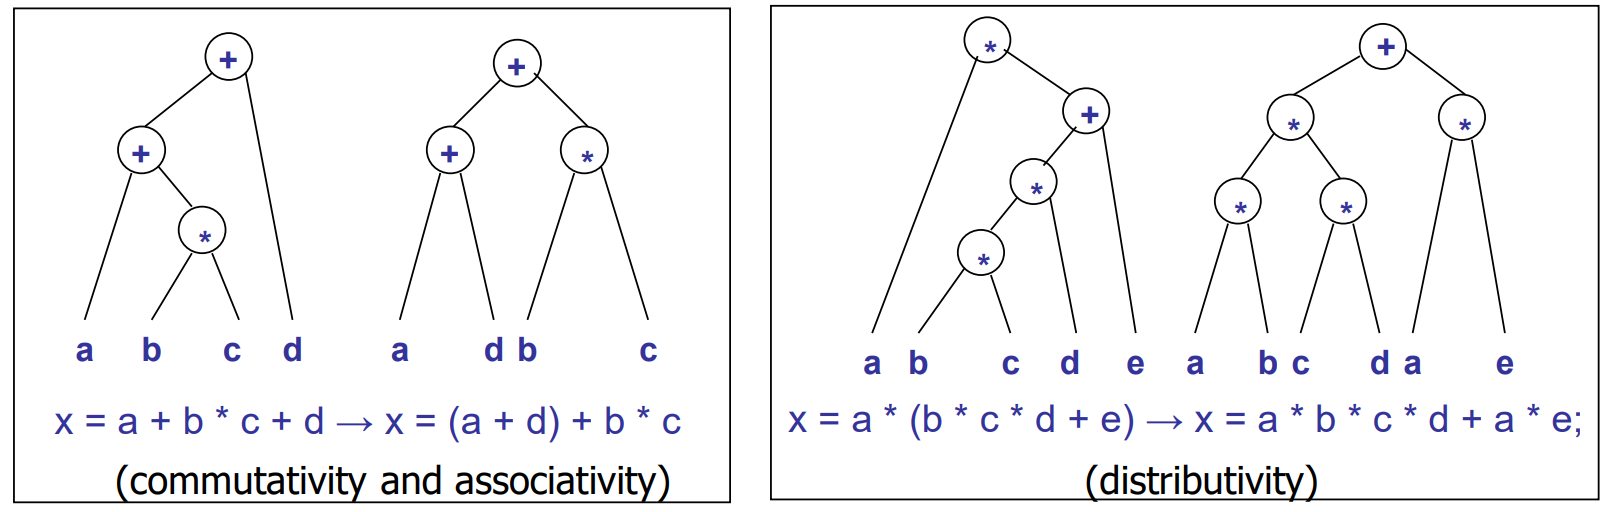
\includegraphics[width=17cm, scale=1]{S2/treeHeightReduction.PNG}
                \caption{Tree-height reduction}
            \end{figure}
        \end{itemize}
    \newpage
    \item Propagation
        \begin{figure}[htp]%
            \centering
            \subfloat[\centering \textit{Constant} propagation; \textit{a} can be evaluated at compile time (instead of runtime)]
                     {{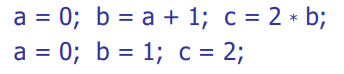
\includegraphics[width=7cm]{S2/constantProp.PNG}}}% 
            \qquad
            \subfloat[\centering \textit{Variable} propagation; \textit{a} and \textit{b} can be evaluated \textbf{simultaneously} now]
                     {{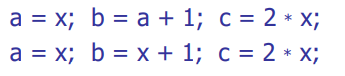
\includegraphics[width=7cm]{S2/variableProp.PNG}}}% 
            \caption{Different propagation techniques}%
        \end{figure}
    \item Sub-expression elimination
        \begin{figure}[htp]%
            \centering
            \subfloat[\centering \textit{Logic} expressions can be simplified with K-Maps]
                     {{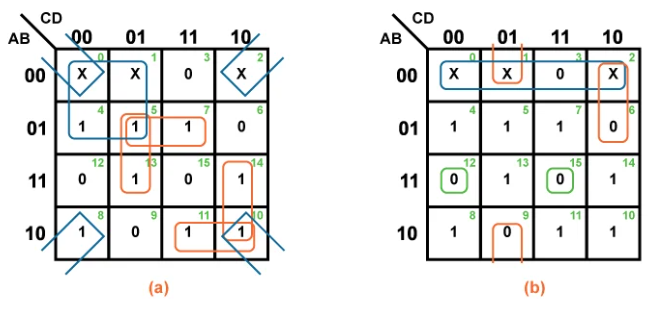
\includegraphics[width=6cm]{S2/kmap}}}% 
            \qquad
            \subfloat[\centering \textit{Arithmetic} expressions can be simplified (like memoization)]
                     {{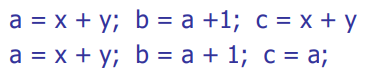
\includegraphics[width=6cm]{S2/arithmeticElimination.PNG}}}% 
            \caption{Different sub-expression eliminations}%
        \end{figure}
    \item Operator-strength reduction
        \begin{itemize}
            \item Complexity of operations is \dots $\xrightarrow[\text{Increasing level of complexity}]
                                                                 {\text{Assignment; Bitwise logical operations(AND,OR,...); Variable shift/Arithmetic operations; Mult; Div}}$
            \begin{figure}[htp]
                \centering
                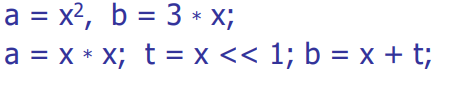
\includegraphics[width=8cm, scale=1]{S2/operatorStrengthReduction.PNG}
                \caption{Use 'weaker' operations if possible}
            \end{figure}
            \item Intuitively, the degree of complexity has to do with how much can be done in parallel
                \begin{itemize}
                    \item Suppose we perform bitwise AND between two 8bit inputs.
                            The operations on each bit can be done \textbf{independently}, which makes it less 'complex'

                        \begin{minipage}{\linewidth}
                            \centering
                            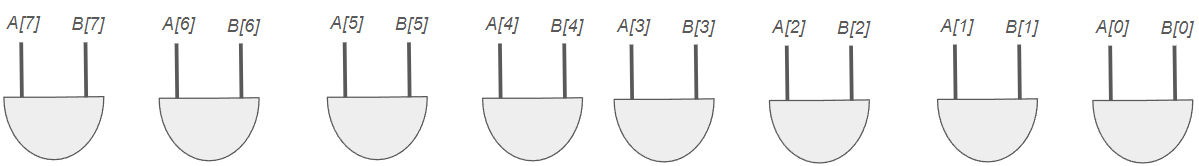
\includegraphics[width=14cm, scale=1]{S2/8bit_AND.PNG}
                            \captionof{figure}{AND operation, done in parallel}
                        \end{minipage}

                    \item Suppose we are performing addition.
                            The operations cannot be done independently, there is data dependency on the carry bit. This makes it more 'complex'

                        \begin{minipage}{\linewidth}
                            \centering
                            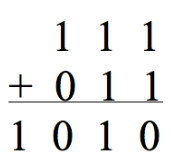
\includegraphics[width=2cm, scale=1]{S2/additionCarry.PNG}
                            \captionof{figure}{Addition operation. Note that we must wait for the carry bit to propagate through}
                        \end{minipage}
                \end{itemize}
        \end{itemize}
\end{itemize}

\newpage
\subsubsection{Some control-flow based transformations}
\begin{itemize}
    \item Modal expansion (ie. Inline function)
        \begin{itemize}
            \item \textit{Flattens} the hierarchy, removing module boundaries and encouraging cross-module optimizations (that would not have been obvious before)
            \item Removes the need for \textit{Program Counter(PC)} to jump abruptly, avoiding control hazards and etc \dots
        \end{itemize}
        \begin{minipage}{\linewidth}
            \centering
            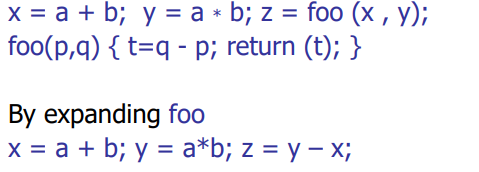
\includegraphics[width=7cm, scale=1]{S2/modalExpansion.PNG}
            \captionof{figure}{Modal expansion}
        \end{minipage}

    \item Conditional expansion
        \begin{itemize}
            \item Very useful for \textbf{logical} expressions, removes the need to evaluate condition during runtime
            \item Note that it may preclude hardware sharing
        \end{itemize}
        \begin{minipage}{\linewidth}
            \centering
            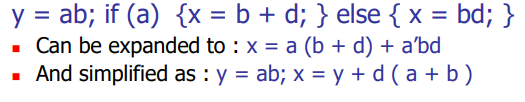
\includegraphics[width=7cm, scale=1]{S2/conditionalExpansion.PNG}
            \captionof{figure}{Conditional expansion. Note that this is a boolean function, not an arithmetic function}
        \end{minipage}

    \item Loop expansion
        \begin{itemize}
            \item Applicable to loops with data-\textbf{independent} exit conditions
        \end{itemize}
        \begin{figure}[htp]
            \centering
            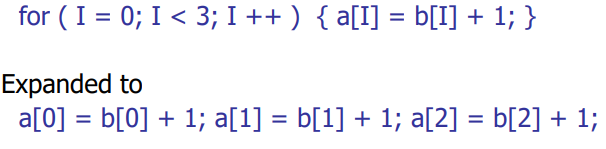
\includegraphics[width=11cm, scale=1]{S2/loopExpansion.PNG}
            \caption{Loop unrolling}
        \end{figure}
\end{itemize}

\subsection{Architectural Synthesis}
\textbf{Implementation} of \textit{structural} design from (behaviorally optimized) \textit{behavioral} CDFGs.

More formally, we can \textit{synthesize} a \textbf{macroscopic} structure because we have \dots
\begin{enumerate}
    \item Circuit behavior (Sequencing graph)
    \item Cells ('Building blocks') from technology library, fully characterized in terms of area and execution delay
    \item Timing and area/resource usage constraints; Which will be utilized to do scheduling and binding
\end{enumerate}

\begin{figure}[htp]
    \centering
    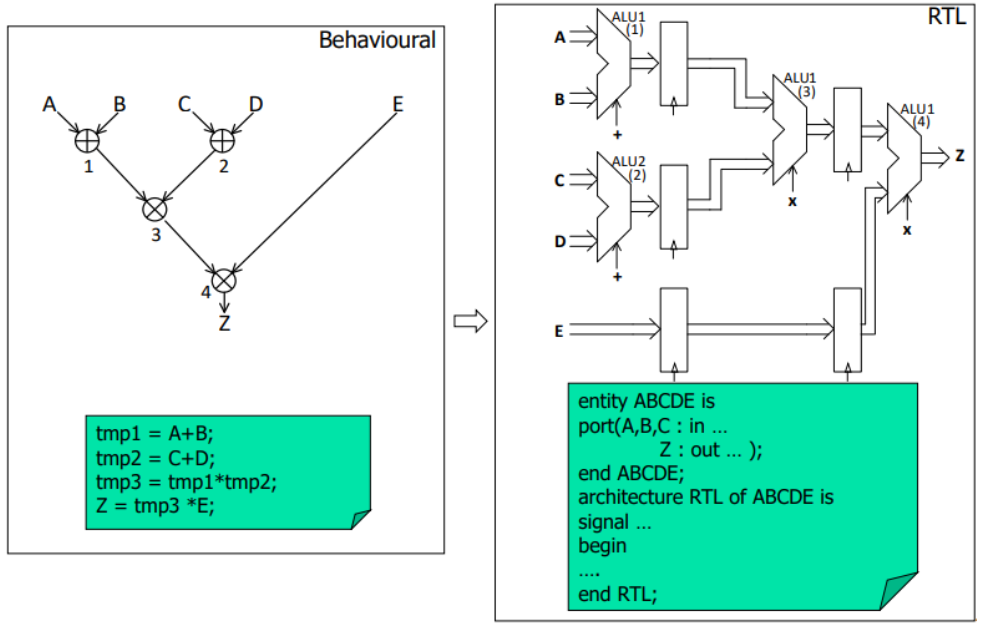
\includegraphics[width=9cm, scale=1]{S2/architecturalSynthesis.PNG}
    \caption{Behavioral to Structural}
\end{figure}

\subsubsection{Technology library cells}
Can be broadly split into \textit{data-path} and \textit{control-unit} cells

\begin{minipage}[t]{0.5\textwidth}
    Data-path cells consist of \dots
    \begin{itemize}
        \item Arithmetic and logic blocks
            \begin{itemize}
                \item Functional units that perform operations on data
            \end{itemize}
        \item Memory and registers
            \begin{itemize}
                \item Storage resources to store data
            \end{itemize}
        \item External buses and ports
            \begin{itemize}
                \item Interconnection of different blocks together
            \end{itemize}
        \item Muxes and \textbf{internal} buses
            \begin{itemize}
                \item Steering logic to appropriately channel data \textbf{within} a block
            \end{itemize}
    \end{itemize}
\end{minipage}%
\begin{minipage}[t]{0.5\textwidth}
    Control-unit cells need to control the flow of data \textbf{within} the datapath, utilizing \dots
    \begin{itemize}
        \item Mux \textit{selects}
        \item Register write-\textit{enable}s
        \item Functional unit \textit{activation}/\textit{enable}, and operation \textit{selection} signals
    \end{itemize}
\end{minipage}%

\subsubsection{Implementation constraints}
Can be broadly split into \textit{timing} constraints and \textit{resource} constraints

Timing constraints could come in the form of \dots
\begin{itemize}
    \item Cycle-time
        \begin{itemize}
            \item What is the frequency that your circuit should operate at?
                \begin{itemize}
                    \item If we have single-cycle operations, then the logic must have it's result by the next clock edge
                    \item Multi-cycle operations (eg. pipelined computations) relax the above constraint
                \end{itemize}
        \end{itemize}
    \item Latency between a set of operations (ie. Set of operations must complete within 'x' amount of cycles)
    \item Time spacing between operation pairs (ie. Operations must be spaced 'x' amount of cycles apart)
\end{itemize}

Resource constraints could come in the form of \dots
\begin{itemize}
    \item Allocation
        \begin{itemize}
            \item Only given limited number of functional units to achieve some functionality
        \end{itemize}
    \item Partial binding (ie. some operations are unalterably tied to some functional units)
\end{itemize}

\subsubsection{Scheduling and Binding - Overview}
In architectural synthesis, we have an area/performance trade-off.

An optimal implementation will maximize performance subject to area constraints (or vice versa). But how do we achieve this optimal implementation?

This is done via \textit{scheduling} and \textit{binding}. 
Place vertices of CDFG (representing operand-operations) in \dots
\begin{itemize}
    \item Time (Scheduling); Determine which operand-operation occurs during each clock cycle 
    \item Space (Binding); Determine which hardware resource should be utilized 
        \begin{itemize}
            \item Map operand-operations to functional units (\textit{Function binding})
            \item Map variables to storage units (\textit{Storage binding})
            \item Map data transfers to buses (\textit{Connection binding})
        \end{itemize}
\end{itemize}

\newpage
\subsubsection{Scheduling}
When doing scheduling (ie. Synthesis in the \textit{temporal} domain) on a CDFG graph, the \dots
\begin{itemize}
    \item Edges denote the \textit{latency} of the vertex (we assume no edge label means latency of 1)
    \item \textit{Granularity} is in terms of \textit{cycles}, not seconds
\end{itemize}

Scheduling associates a start-time for each operation (vertex) in the sequencing graph.
From this, we can determine the \textit{latency} and \textit{parallelism} of the implementation.

\begin{figure}[htp]
    \centering
    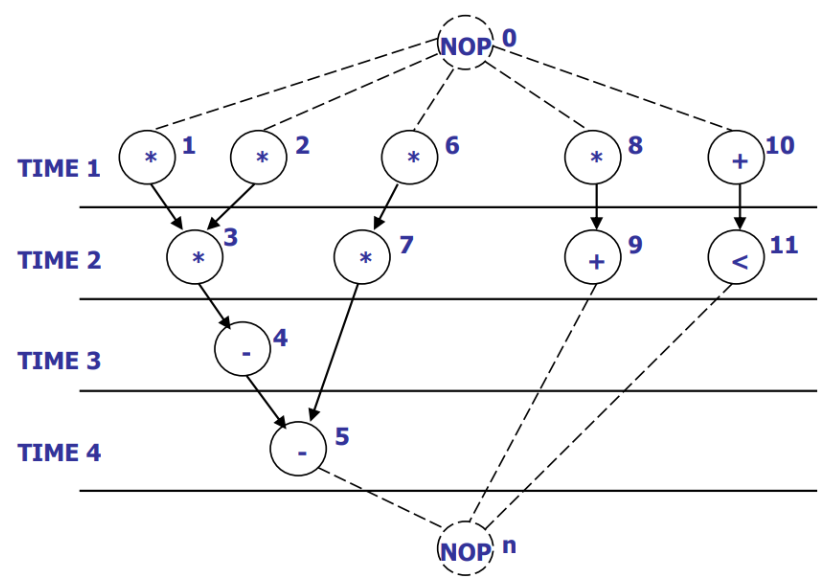
\includegraphics[width=10cm, scale=1]{S2/scheduledSequencingGraph.PNG}
    \caption{Sequencing graph that has been scheduled}
\end{figure}

\paragraph{Mathematical model of scheduling}\mbox{}\\\\
Let's describe scheduling mathematically.

\begin{enumerate}
    \item 
    Define our graph objects \dots
    \begin{itemize}
        \item Vertices $V = \left\{ v_{0}, v_{1}, \dots, v_{n} \right\}$; $v_{0}$ is source node, $v_{n}$ is sink node
        \item Node latencies $M = \left\{ \mu_{0}, \mu_{1}, \dots, \mu_{n} \right\}$ st. $\mu_{i}\in Z$ (Node latency cannot be negative)
        \item Operation start times $T = \left\{ \tau_{0}, \tau_{1}, \dots, \tau_{n} \right\}$ st. $\tau_{i}\in Z^{+}$ (ie. Begin counting from 1)
    \end{itemize}
    \item Then, define the function $\varphi$ : $V \xrightarrow{} Z^{+}$ as $\varphi(v_{i}) = \tau_{i}$ st \dots
        \begin{itemize}
            \item $\tau_{i}$ (denoting the \textit{operation start time}) obeys $\tau_{i} \ge \tau_{j} + \mu_{j}; \ \forall (v_{j},v_{i}) \in \textit{valid edge} $
            \item This is just saying that an operation can only start when it's precedence constraint is fufilled (ie. Operators before it have completed their computation and are ready with results)
        \end{itemize}
    \item \textbf{Overall} latency $\mu_{overall} = \tau_{n} - \tau_{0}$;
    \item Scheduling is the task of optimally determining $T$, subject to precedence constraints specified in the sequencing graph
\end{enumerate}

\newpage
\paragraph{Different kinds of scheduling}\mbox{}\\
\begin{itemize}
    \item ASAP scheduling (Optimize for the lowest $\mu_{overall}$, not factoring in functional unit availability)
        \begin{itemize}
            \item Unconstrained hardware availability (We have infinite functional units)
                \begin{itemize}
                    \item Operation is only delayed by precedence constraints, not by hardware availability
                \end{itemize}
            \item Maximally constrained hardware availability (We have only one of each type of functional unit)
                \begin{itemize}
                    \item We are still optimizing for lowest $\mu_{overall}$. This is actually an NP-hard combinatorial optimization problem.
                \end{itemize}
        \end{itemize}

        \begin{minipage}{0.5\linewidth}
            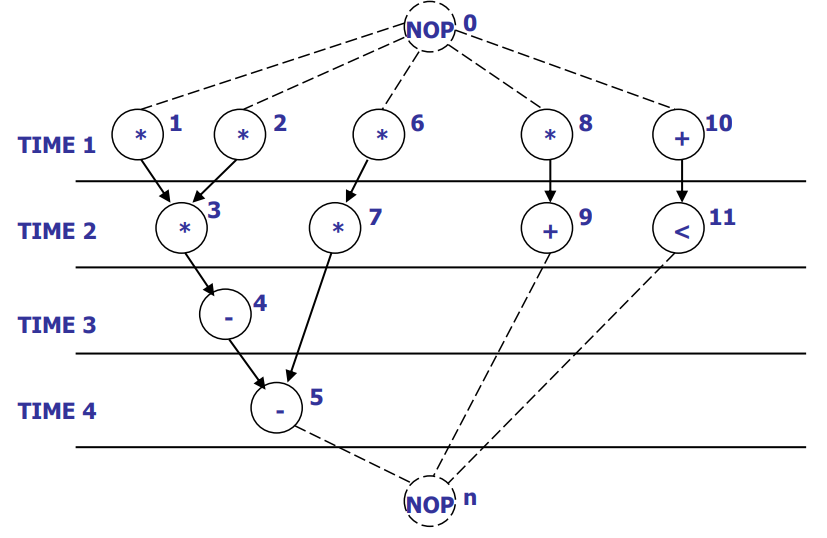
\includegraphics[width=9cm]{S2/asapSchedule1.PNG}
            \captionsetup{justification=centering}
            \captionof{figure}{Unconstrained\\
                                $\mu_{overall} = 5-1 = 4$\\
                                Minimal resource usage: x4 MUL units, x2 ALU units}
        \end{minipage}%
        \hfill
        \begin{minipage}{0.5\linewidth}
            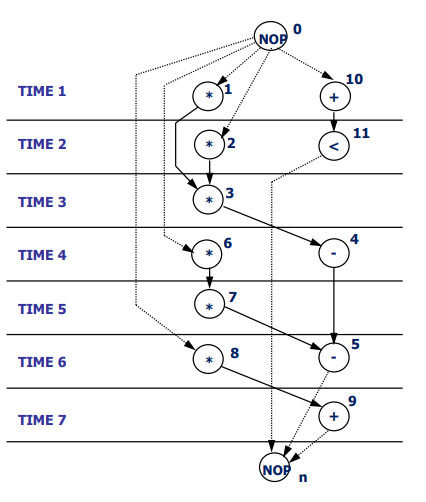
\includegraphics[width=7cm]{S2/asapSchedule2.PNG}
            \captionsetup{justification=centering}
            \captionof{figure}{Maximally constrained\\
                                $\mu_{overall} = 8-1 = 7$\\} 
        \end{minipage}%

    \item ALAP scheduling
        \begin{itemize}
            \item Scheduling under unconstrained-ASAP is equivalent to finding longest path between each vertex and \textbf{source} node.
                \begin{minipage}{0.5\linewidth}
                    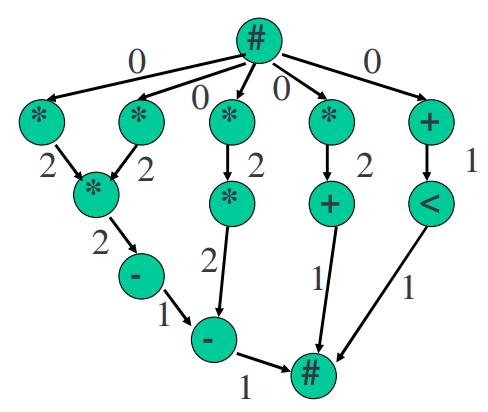
\includegraphics[width=7cm]{S2/alap1.PNG}
                    \captionsetup{justification=centering}
                    \captionof{figure}{Edge-weighted CDFG}
                \end{minipage}%
                \hfill
                \begin{minipage}{0.5\linewidth}
                    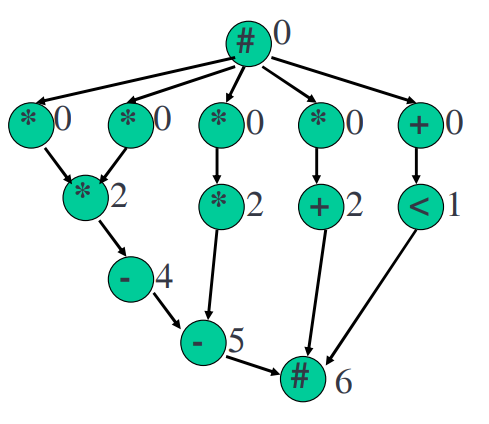
\includegraphics[width=7cm]{S2/alap2}
                    \captionsetup{justification=centering}
                    \captionof{figure}{Applying longest path algorithm leads to ASAP start-times}
                \end{minipage}%
            \vspace{2cm}
            \item Unconstrained-ALAP is then the opposite; We schedule operations at the latest opportunity.
                    This can be performed by seeking the longest path between each vertex and \textbf{sink} node, then subtracting longest path time from desired $\mu_{overall}$

                \begin{minipage}{0.33\linewidth}
                    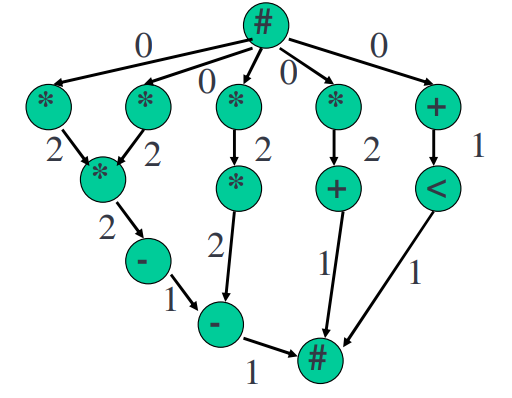
\includegraphics[width=6cm]{S2/alap3.PNG}
                    \captionsetup{justification=centering}
                    \captionof{figure}{Edge-weighted CDFG}
                \end{minipage}%
                \hfill
                \begin{minipage}{0.33\linewidth}
                    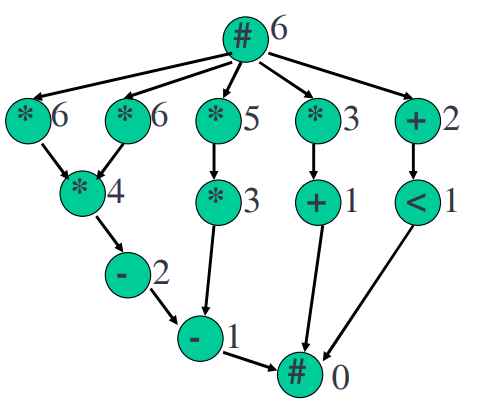
\includegraphics[width=6cm]{S2/alap4}
                    \captionsetup{justification=centering}
                    \captionof{figure}{Longest path to sink node}
                \end{minipage}%
                \hfill
                \begin{minipage}{0.33\linewidth}
                    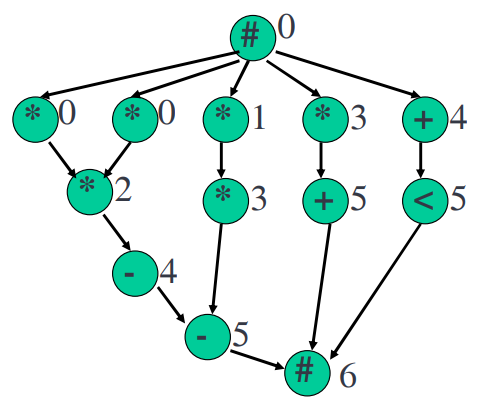
\includegraphics[width=6cm]{S2/alap5}
                    \captionsetup{justification=centering}
                    \captionof{figure}{Supposing $\mu_{overall} = 6$}
                \end{minipage}%
                \vspace{0.5cm}

            \item The difference between ALAP and ASAP time for a \textbf{vertex} is termed the \textit{operation mobility} or \textit{slack}.
            
                    Mobility measures how free we are to move vertices into different time-slots. Operations with zero mobility are \textit{critical} operations,
                    and together they form the \textit{critical path}, which determines how fast our circuit can run.
            \end{itemize}

    \item Scheduling with chaining
            \begin{itemize}
                \item What if we allow two or more \textbf{combinational} operations to execute in the same cycle?
                \item In the example below, suppose \dots
                    \begin{itemize}
                        \item Mult: 35s
                        \item Others: 25ns
                        \item Cycle time: 50ns
                    \end{itemize}
                \item Then, we can squeeze x2 ALU units back-to-back into a single clock cycle
                \item Note that the latency has decreased, but now we require x2 ALUs minimally
                \item Note also that there is a cycle-time and latency tradeoff. Compared to Fig25, we notice that Fig33 has a longer cycle-time (but shorter latency)
            \end{itemize}
    
            \begin{minipage}{\linewidth}
                \centering
                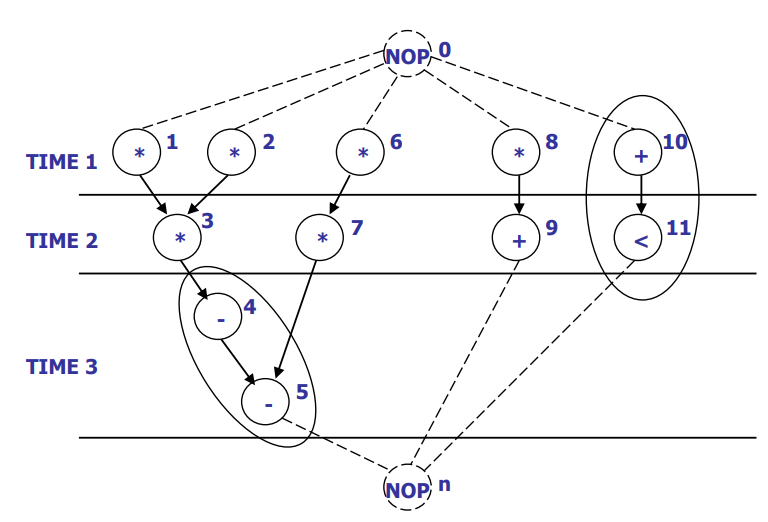
\includegraphics[width=14cm, scale=1]{S2/chaining.PNG}
                \captionof{figure}{Chained operations}
            \end{minipage}

\end{itemize}

\newpage
\subsubsection{Binding}
When doing binding (ie. Synthesis in the \textit{spatial} domain) on a \textbf{scheduled} CDFG graph, we \dots
\begin{itemize}
    \item Associate a resource (described as a \textbf{2-tuple} (\textit{type}, \textit{instance}) annotation beside the vertex) with each operation.
        From this, we can determine the \textit{area} of implementation.
        \begin{itemize}
            \item \textit{Type} denotes the type of functional unit (eg. ALU, Adder, MUL, ...)
            \item \textit{Instance} denotes the instance of a \textbf{specific type} of functional unit. (eg. ALU1, ALU2, ...)
        \end{itemize}
    \item Operations bound to the same resource, belong to the same hypergraph.
\end{itemize}

\begin{figure}[htp]
    \centering
    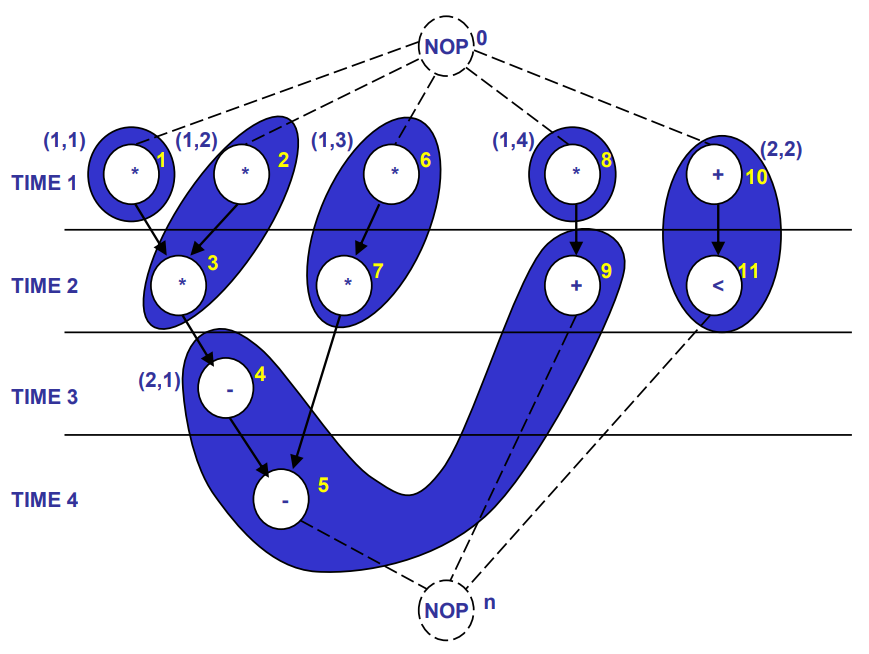
\includegraphics[width=12cm, scale=1]{S2/bindingGraphExample.PNG}
    \caption{Binding a scheduled sequencing graph}
\end{figure}

The key point to notice is that when we bind a resource to more than one operation, the operations must not execute concurrently.
Intuitvely this makes sense, since the same hardware cannot be shared amongst two operations in the same clock cycle.

\paragraph{Mathematical model of Binding}\mbox{}\\\\
Let's describe binding mathematically.

\begin{enumerate}
    \item 
    Define our graph objects \dots
    \begin{itemize}
        \item Vertices $V = \left\{ v_{1}, v_{2}, \dots, v_{n} \right\}$; $v_{0}$ is source node, $v_{n}$ is sink node
        \item Types $Q = \left\{ q_{1}, q_{2}, \dots, q_{num\_types} \right\}$
        \item Instances (\textbf{of a specific type} $q_{i}$) $R = \left\{ r_{1}, r_{2}, \dots, r_{num\_instances} \right\}$ st. $r_{i} \in Z^{+}$
    \end{itemize}
    \item Define \textit{resource binding} \textbf{function} $\beta$ : $V \xrightarrow{} Q\times Z^{+}$ as $\beta(v_{i}) = (q_{i},r_{i})$
        \begin{itemize}
            \item Plainly, $\beta(v_{i}) = (q_{i},r_{i})$ means an operation (corresponding to $v_{i}$) is implemented
                    by the $r_{i}^{th}$ instance of functional unit type $q_{i}$
            \item $\beta$ is \textit{one-to-one} $\longrightarrow$ We have dedicated binding
                \begin{itemize}
                    \item One instance of one functional unit type, implements only one vertex
                \end{itemize}
            \item $\beta$ is \textit{many-to-one} $\longrightarrow$ Resource sharing \textbf{is} happening
                \begin{itemize}
                    \item Multiple vertices are mapped to the same resource (ie. same instance of same functional unit type)
                \end{itemize}
        \end{itemize}
    \item Define \textit{implementation} \textbf{relation} $\theta$ : $V \xrightarrow{} Q$ as $\theta(v_{i}) = q_{i}$ st. $q_{i} \in Q$
        \begin{itemize}
            \item Plainly, $\theta(v_{i}) = q_{i}$ means that the $i^{th}$ operation is implemented by functional unit type $q_{i}$
            \item $\theta$ is \textit{one-to-many} $\longrightarrow$ We have a choice of \textit{which} functional unit type we wish to utilize
                \begin{itemize}
                    \item eg. If $v_{i}$ is an addition operation, it could be implemented by ALU or Adder functional unit
                \end{itemize}
            \item $\theta$ is \textit{many-to-one} $\longrightarrow$ Multiple operations are mapped to the same functional unit type, resource sharing is \textbf{possible} (not \textbf{confirmed})
                \begin{itemize}
                    \item Suppose that operations $v_{i}$ and $v_{j}$ do not overlap. Then they can both use the same instance of the same functional unit type $q_{k}$, which is resource sharing.
                    \item Suppose that operations $v_{i}$ and $v_{j}$ overlap. Then they must use different instances of the same functional unit type $q_{k}$, meaning resource sharing is not possible
                \end{itemize}
        \end{itemize}
\end{enumerate}

\paragraph{Example of binding}\mbox{}\\
\begin{figure}[htp]
    \centering
    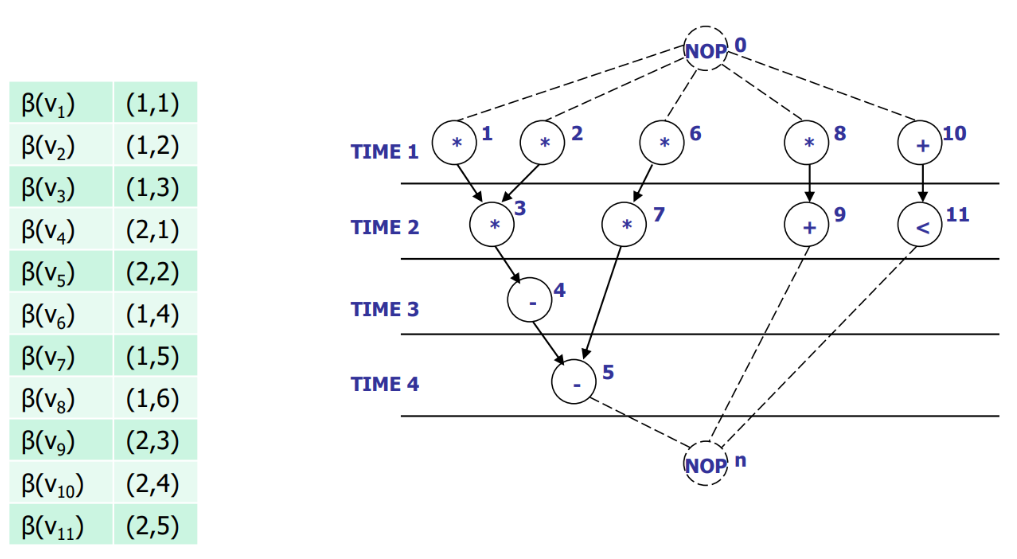
\includegraphics[width=12cm, scale=1]{S2/binding1.PNG}
    \caption{Dedicated binding\\
            6 MULs, 5 ALUs}
\end{figure}

\begin{minipage}{0.6\linewidth}
    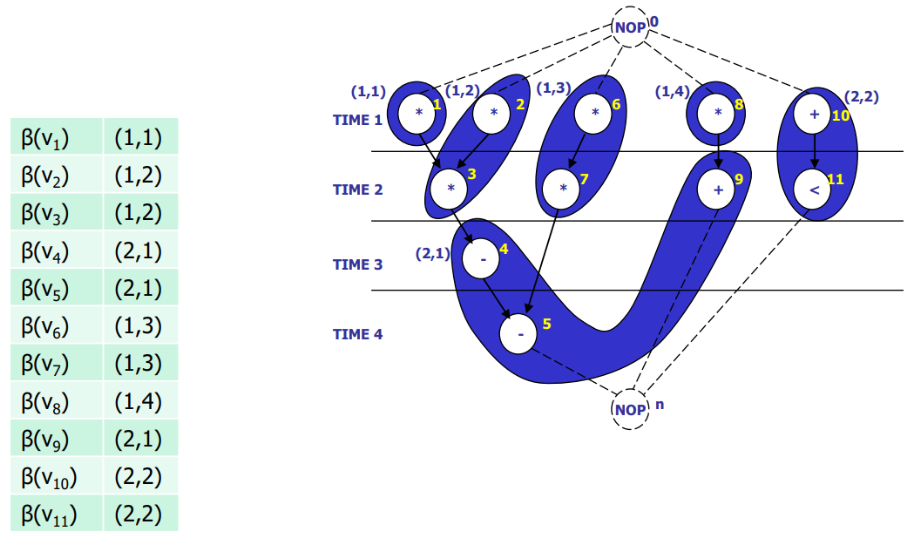
\includegraphics[width=12cm]{S2/binding2.PNG}
    \captionsetup{justification=centering}
    \captionof{figure}{Binding with resource sharing\\
                        4 MULS, 2 ALUs}
\end{minipage}%
\hfill
\begin{minipage}{0.4\linewidth}
    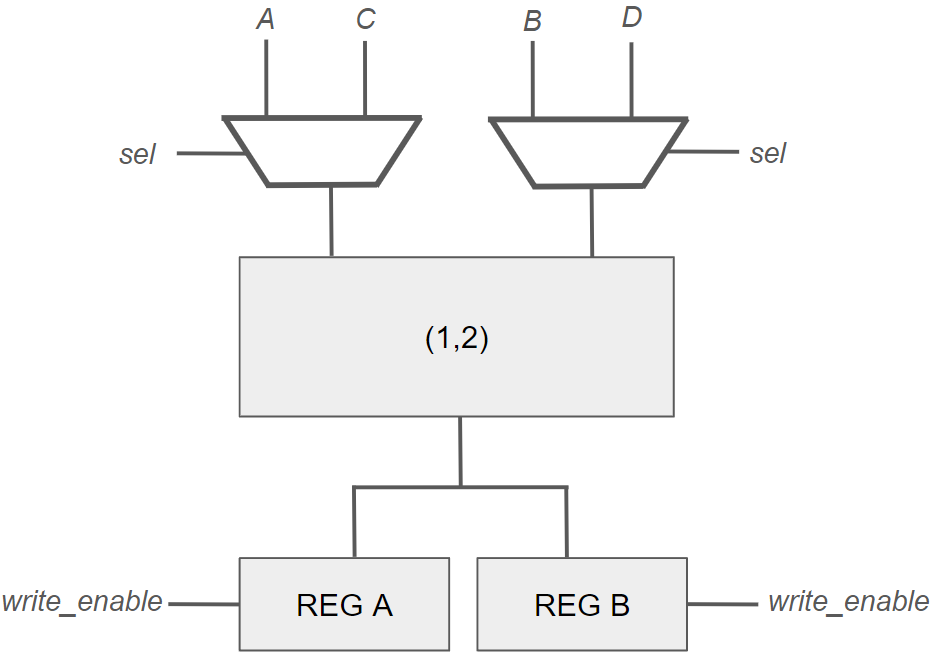
\includegraphics[width=8cm]{S2/complicatedControl.PNG}
    \captionsetup{justification=centering}
    \captionof{figure}{More complex control logic}
\end{minipage}%


Resource sharing means that multiplexers and registers need more complicated control signals to manage dataflow.
Therefore, a major benefit of utilizing dedicated binding is that it results in greatly simplified control logic.

Consider vertices 2 and 3 in Fig36. 
Suppose vertex 2 is a (A*B) operation, vertex 3 is a (C*D) operation. 
We can observe that due to resource-sharing, the shared (1,2) MUX functional unit requires multiplexers (with appropriate \textit{sel} to select which data to operate on), as well as different registers (with different \textit{write enables} to store data)

\newpage
\section{Data-path Synthesis, Control-path Synthesis}
Once a complete binding has been done, we will need to synthesize our Data-path and Control-path as the last step

\subsection{Data-path Synthesis}
\begin{itemize}
    \item Defining the interconnection amongst \dots
        \begin{itemize}
            \item Functional units (Multiplier, ALU, etc...)
            \item Steering resources (MUXs, Buses)
            \item Memory Resources (Registers, Memory arrays)
            \item \textbf{Data-dependent} condition signals (ie. Branching, iteration)
        \end{itemize}
\end{itemize}

\begin{figure}[htp]
    \centering
    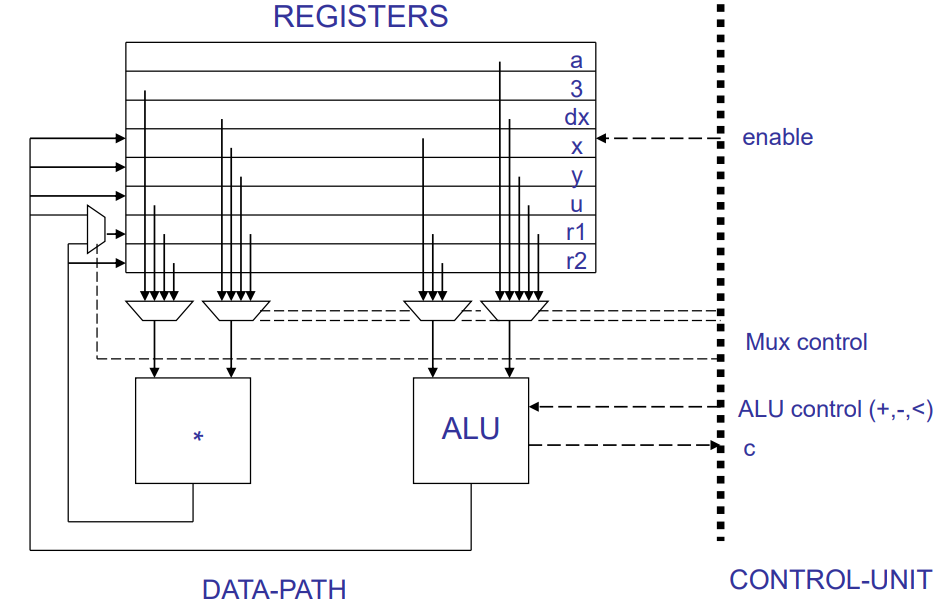
\includegraphics[width=14cm, scale=1]{S3/dataPathSynthesis.PNG}
    \caption{Datapath for 1 MUX, 1 ALU system\\
                Only 2 intermediate variables at any one time, stored in $r1$ and $r2$}
\end{figure}

\subsection{Control-path Synthesis}
Suppose we want to synthesize the control signals for the scheduled graph below

\begin{figure}[htp]
    \centering
    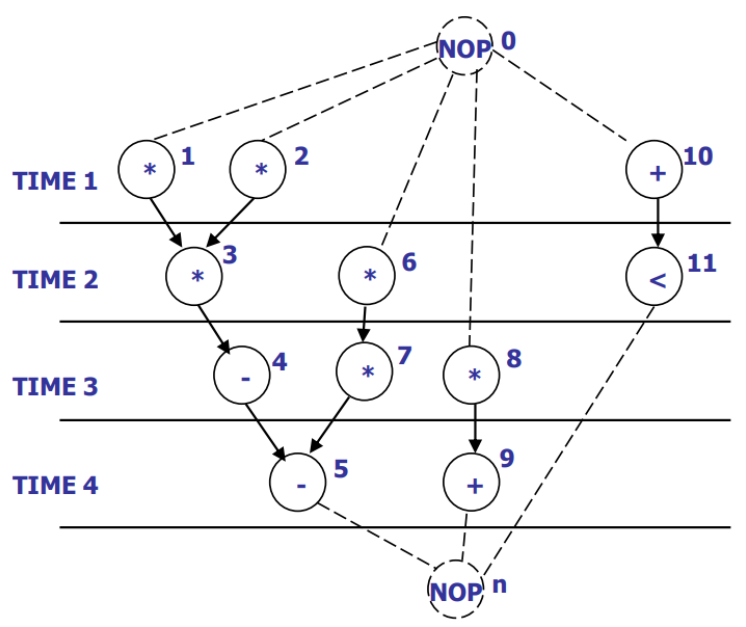
\includegraphics[width=8cm, scale=1]{S3/controlPathSynthesis1.PNG}
    \caption{Assume dedicated binding (for simplicity)}
\end{figure}

There are two ways to do it - Hardwired FSM or Microcode.

\newpage
\subsubsection{Hardwired FSM}
Classical state machine that we are used to

\begin{figure}[htp]
    \centering
    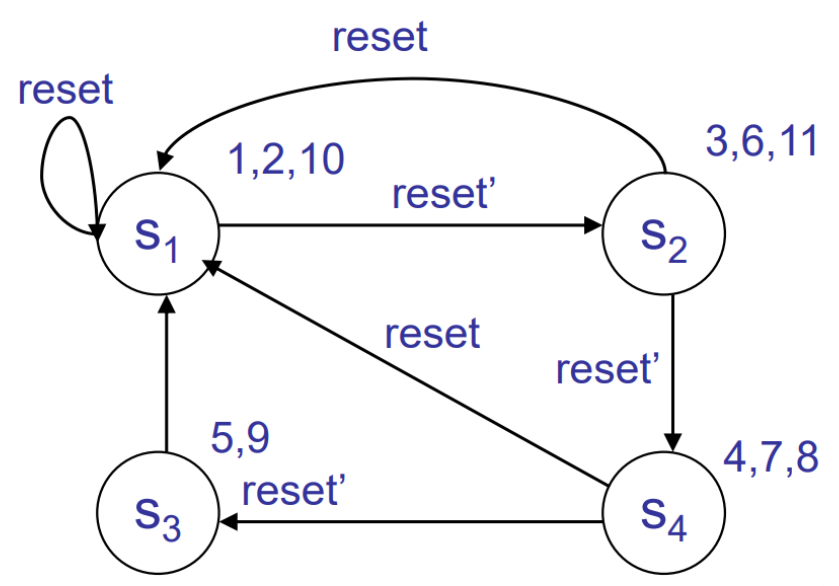
\includegraphics[width=8cm, scale=1]{S3/hardwiredFSM.PNG}
\end{figure}

\subsubsection{Microcode}

\begin{itemize}
    \item One activation signal per resource (thus 11 bits required for 11 resources)
    \item 4 states (each potentially controlling up to 11 resources) requires $log_{2}(4) = 2$ bit ROM counter
\end{itemize}

\paragraph{Horizontal Microcode}\mbox{}\\
\begin{figure}[htp]
    \centering 
    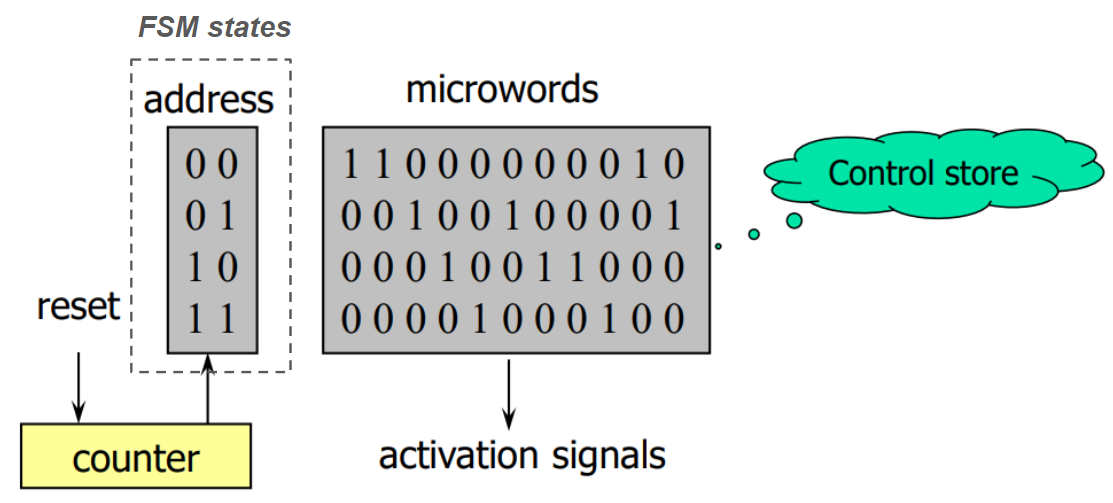
\includegraphics[width=10cm, scale=1]{S3/horizontalMicrocode.PNG}
\end{figure}

\paragraph{Vertical Microcode}\mbox{}\\
We can \textit{compress} horizontal microcode (which suffers from sparsity) to form \textit{vertical microcode}
\begin{itemize}
    \item Allows only one resource to be activated per time-step (if memory is single-port), which can be solved by either \dots
        \begin{itemize}
            \item Lengthening the schedule
            \item Reading multiple microcodes per schedule step (requires multi-port memory)
        \end{itemize}
\end{itemize}

\begin{minipage}{0.5\linewidth}
    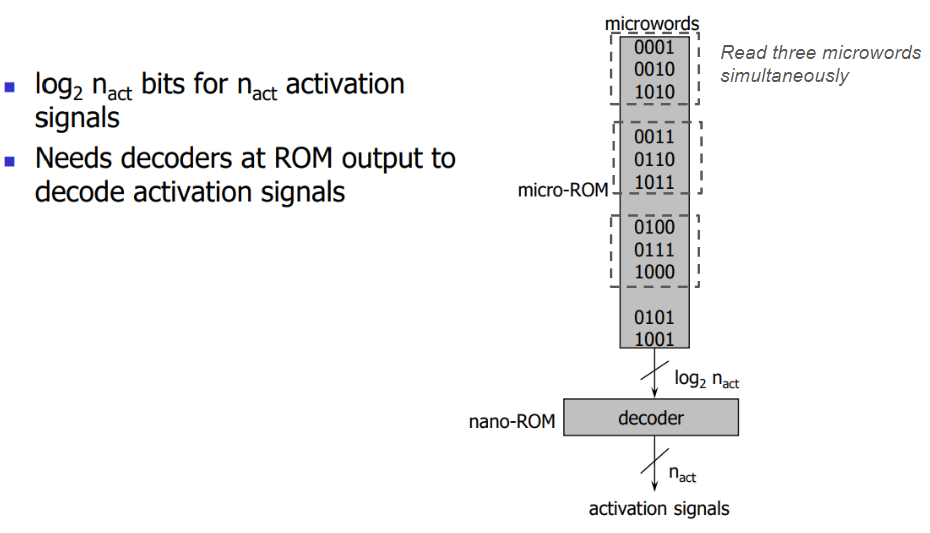
\includegraphics[width=9cm, scale=1]{S3/verticalMicrocode.PNG}
    \captionsetup{justification=centering}
    \captionof{figure}{Vertical Microcode\\
                        eg. \textit{1010} means that we want to activate resource 10}
\end{minipage}%
\hfill
\begin{minipage}{0.5\linewidth}
    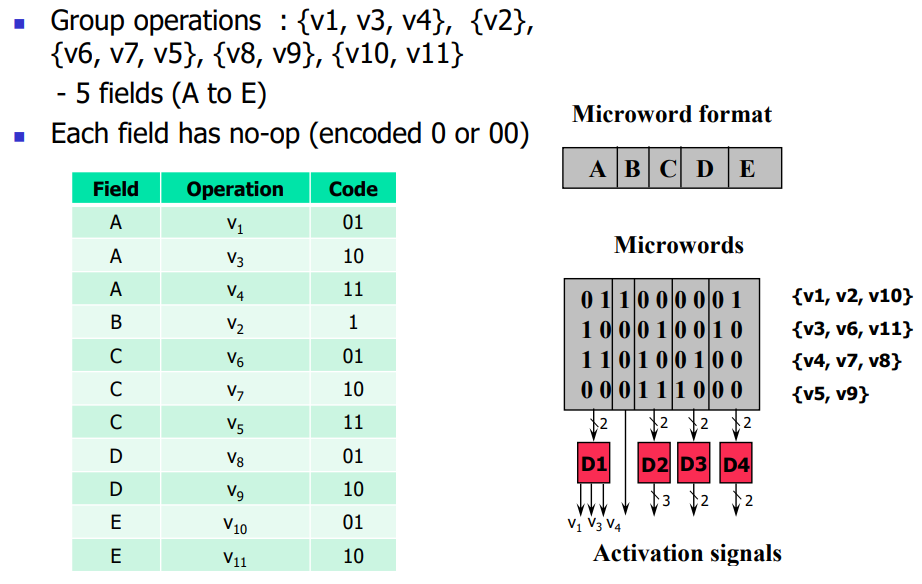
\includegraphics[width=10cm, scale=1]{S3/verticalMicrocodeGrouping.PNG}
    \captionsetup{justification=centering}
    \captionof{figure}{Vertical Microcode with Grouping}
\end{minipage}%

\end{document}